\documentclass[a4paper,10pt]{article}

\usepackage{ucs}
\usepackage[utf8]{inputenc}
\usepackage[spanish]{babel}
\usepackage{fontenc}
\usepackage{graphicx}
\usepackage{enumerate}
\author{Roberto Castellor Morant}
\title{Ped 2 sistemas en tiempo real}
\date{\today}

\begin{document}
\maketitle


\section{Ejercicio 2}

Considérese un sistema que tiene cinco recursos (P1, P2, P3, P4, P5) y siete
recursos (R1, R2, R3, R4, R5, R6, R7). Hay una instancia de los recursos 2, 5 
y 7, y dos instancias de los recursos 1, 3, 4 y 6. El proceso 1 tiene asignada
una instancia de R1 y requiere una de R7.  El proceso 2 tiene asignadas una 
instancia de R1, R2 y R3 y requiere una de R5. El proceso 3 tiene asignada una 
instancia de R3 y R4 y requiere una de R1. El proceso 4 tiene asignada R4 y R5 
y requiere una de R2. El proceso 5 tiene una de R7.


Estudio si este sistema se encuentra en una situación de interbloqueo, y 
explique sus razones.

\section{Respuesta PED 2}
Para que el proceso se encuentre en situación de interbloqueo debe cumplir
cuatro condiciones necesarias:

\begin{itemize}
	\item Condición de exclusión mutua, existe un recurso compartido por los
procesos al que solo puede acceder un proceso simultaneamente, los recursos 2, 5
y 7 cumplen esta condición
	\item Condición de retención y espera, al menos un proceso P ha
adquirido un recurso R y lo retiene mientras espera un recurso R2 que ha sido
asignado a otro proceso. El proceso 4 tiene adquirido el recurso R5 mientras
espera el recurso R2 que está bloqueado por el proceso 2.
	\item Condición de no expropiación, los recursos no pueden ser
expropiados por otros procesos, tienen que ser liberados por sus propietarios.
	\item Condición de espera circular, el proceso P2 tiene bloqueada la
unica instancia del recurso 2, requiere la instancia del recurso R5 que esta
bloqueada por el proceso 4 y que a su vez requiere el recurso 2 por lo que se
produce una situación de retención y espera.


		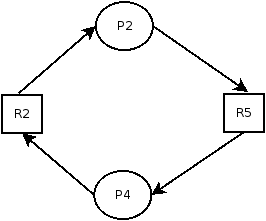
\includegraphics{condicion_circular}
\end{itemize}

En el escenario mostrado se cumplen las cuatro condiciones necesarias por lo que
podemos afirmar que hay un bloqueo
\end{document}
